%%%%%%%%%%%%%%%%%%%%%%%%%%%%%%%%%%%%%%%%%%%%%%%%%%%%%%%%%%%%%%%
%
% Welcome to Overleaf --- just edit your LaTeX on the left,
% and we'll compile it for you on the right. If you open the
% 'Share' menu, you can invite other users to edit at the same
% time. See www.overleaf.com/learn for more info. Enjoy!
%
%%%%%%%%%%%%%%%%%%%%%%%%%%%%%%%%%%%%%%%%%%%%%%%%%%%%%%%%%%%%%%%

% Inbuilt themes in beamer
\documentclass{beamer}

%packages:
% \usepackage{tfrupee}
% \usepackage{amsmath}
% \usepackage{amssymb}
% \usepackage{gensymb}
% \usepackage{txfonts}

% \def\inputGnumericTable{}

% \usepackage[latin1]{inputenc}                                 
% \usepackage{color}                                            
% \usepackage{array}                                            
% \usepackage{longtable}                                        
% \usepackage{calc}                                             
% \usepackage{multirow}                                         
% \usepackage{hhline}                                           
% \usepackage{ifthen}
% \usepackage{caption} 
% \captionsetup[table]{skip=3pt}  
% \providecommand{\pr}[1]{\ensuremath{\Pr\left(#1\right)}}
% \providecommand{\cbrak}[1]{\ensuremath{\left\{#1\right\}}}
% %\renewcommand{\thefigure}{\arabic{table}}
% \renewcommand{\thetable}{\arabic{table}}      

\setbeamertemplate{caption}[numbered]{}

\usepackage{enumitem}
\usepackage{tfrupee}
\usepackage{amsmath}
\usepackage{amssymb}
\usepackage{gensymb}
\usepackage{graphicx}
\usepackage{txfonts}

\def\inputGnumericTable{}

\usepackage[latin1]{inputenc}                                 
\usepackage{color}                                  \usepackage{textcomp, gensymb}         
\usepackage{array}                                            
\usepackage{longtable}                                        
\usepackage{calc}                                             
\usepackage{multirow}                                         
\usepackage{hhline}                             
\usepackage{mathtools}
\usepackage{ifthen}
\usepackage{caption} 
\providecommand{\pr}[1]{\ensuremath{\Pr\left(#1\right)}}
\providecommand{\cbrak}[1]{\ensuremath{\left\{#1\right\}}}
\renewcommand{\thefigure}{\arabic{table}}
\renewcommand{\thetable}{\arabic{table}}   
\providecommand{\brak}[1]{\ensuremath{\left(#1\right)}}

% Theme choice:
\usetheme{CambridgeUS}

% Title page details: 
\title{Assignment 9} 
\author[CS21BTECH11017]{G HARSHA VARDHAN REDDY (CS21BTECH11017)}
\date{\today}
\logo{\large{AI1110}}


\begin{document}

% Title page frame
\begin{frame}
    \titlepage 
\end{frame}
\logo{}


% Outline frame
\begin{frame}{Outline}
    \tableofcontents
\end{frame}

%\section{Abstract}
%\begin{frame}{Abstract}
%\begin{block}{} This document contains $3^{rd}$ %problem from the chapter $5$ in the book %\textbf{Papoulis Pillai Probability Random %Variables and Stochastic Processes.}
%\end{block}

%\end{frame}


\section{Problem Statement}
\begin{frame}{Problem Statement}

    \begin{block} {Papoulis Pillai Probability Random Variables and Stochastic Processes\\ 
    Exercise : 5-3} If the random variable $x$ is $N(0,c^2)$ and $g(x)$ is a function defined below,  find and sketch the
     distribution and the density of the random variable $y=g(x)$.
     %\blockcolor{grey}
    \begin{align}
        g(x)=
    \begin{dcases}
        x+c & x < -c \\
        0 & -c \leq x \leq c \\
        x-c & x > c \\
    \end{dcases}
    \label{1}
    \end{align}
    \end{block}
    
\end{frame}


\section{Gaussian random variable}

\begin{frame}{Distribution and density functions}
\begin{block}{Probability density function}
    Probability density function $f_X(x)$ for a Normal or Gaussian random variable $N(\mu,\sigma^2)$ is 
    \begin{align}
    f_X(x)&=\frac{1}{\sqrt{2\pi\sigma^2}} e^{\frac{-(x-\mu)^2}{2\sigma^2}}, -\infty \leq x \leq \infty
    \label{2}
\end{align}
\end{block}

\begin{block}{Probability distribution function or Distribution function}
    If $f_X(x)$ is probability density function of a random variable X, then it's corresponding Probability distribution function $F_X(x)$ is 
    \begin{align}
        F_X(x) &= \int_{-\infty}^{x} f_X(x) \, dx \label{eq3}
    \end{align}
\end{block}

\end{frame}


\section{Solution}
\begin{frame}{Solution}
Given,\\
The random variable     $X = N(0,c^2)$\\
\vspace{5pt}
Comparing $N(0,c^2)$ and $N(\mu,\sigma^2)$
\begin{align}
    \mu &= 0 \label{4}\\
    \sigma &= c\label{5}
\end{align}
Therefore, from \eqref{2}, \eqref{4} and \eqref{5}
\begin{align}
    f_X(x)=\frac{1}{\sqrt{2\pi c^2}} e^{\frac{-x^2}{2c^2}}, -\infty \leq x \leq \infty \label{6}
\end{align}
\end{frame}

\begin{frame}{}
Let's find probability distribution function of the random variable $Y=g(x)$
 
\begin{itemize}
    \item If $y > 0$
    \begin{align}
        F_Y(y)&=P(Y\leq y)=P(X-c \leq y)\\
            &=P(X \leq y+c)=F_X(y+c)\\
            &=\int_{-\infty}^{y+c} f_X(t) \, dt \\
            \implies F_Y(y)&=\frac{1}{\sqrt{2\pi c^2}}\int_{-\infty}^{y+c}e^{\frac{-t^2}{2c^2}}\, dt\\
            &=\frac{1}{c\sqrt{2\pi}}\frac{\sqrt{\pi c}}{\sqrt{2}} \left(erf\left(\frac{y+c}{\sqrt{2c}}\right)+1\right)\\
            &=\frac{1}{2\sqrt{c}}\left(erf\left(\frac{y+c}{\sqrt{2c}}\right)+1\right)
    \end{align}
\end{itemize}
\end{frame}

\begin{frame}{}
\begin{itemize}
    \item If $y \leq 0$
    \begin{align}
        F_Y(y)&=P(Y\leq y)=P(X+c \leq y)\\
            &=P(X \leq y-c)=F_X(y-c)\\
            &=\int_{-\infty}^{y-c} f_X(t) \, dt \\
            \implies F_Y(y)&=\frac{1}{\sqrt{2\pi c^2}}\int_{-\infty}^{y-c}e^{\frac{-t^2}{2c^2}}\, dt\\
            &=\frac{1}{c\sqrt{2\pi}}\frac{\sqrt{\pi c}}{\sqrt{2}} \left(erf\left(\frac{y-c}{\sqrt{2c}}\right)+1\right)\\
            &=\frac{1}{2\sqrt{c}}\left(erf\left(\frac{y-c}{\sqrt{2c}}\right)+1\right)
    \end{align}
\end{itemize}

\end{frame}
\begin{frame}{}
Therefore,
\begin{align}
    F_Y(y)&=
        \begin{dcases}
        \frac{1}{2\sqrt{c}}\left(erf\left(\frac{y-c}{\sqrt{2c}}\right)+1\right) & y \leq 0 \\
        \frac{1}{2\sqrt{c}}\left(erf\left(\frac{y+c}{\sqrt{2c}}\right)+1\right) & y > 0
    \end{dcases}
\end{align}
As 
\begin{align}
    f_Y(y)&=\frac{d\left(F_Y(y)\right)}{dy}\\
    f_Y(y)&=
    \begin{dcases}
        \frac{1}{\sqrt{2\pi c^2}} e^{-\frac{(y-c)^2}{2c^2}} & y \leq 0 \\
        \frac{1}{\sqrt{2\pi c^2}} e^{-\frac{(y+c)^2}{2c^2}} & y > 0 \\
    \end{dcases}
\end{align}
\end{frame}
\section{graphs}
\begin{frame}{Probability density function}
If $y<0$
    \begin{figure}[h]
    \centering
    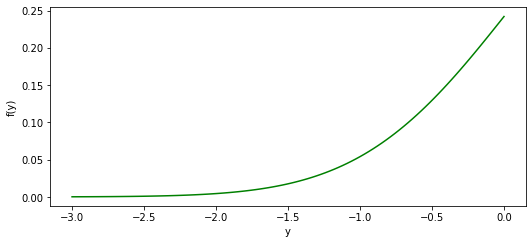
\includegraphics[width=\columnwidth]{figures/f1.png}
    \caption{$f_Y(y)$}
    \label{Fig 1}
    \end{figure}
\end{frame}
\begin{frame}{Probability density function}
If $y \ge 0$
    \begin{figure}[h]
    \centering
    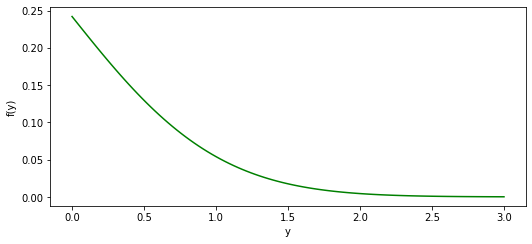
\includegraphics[width=\columnwidth]{figures/f2.png}
    \caption{$f_Y(y)$}
    \label{Fig 2}
    \end{figure}
\end{frame}
\begin{frame}{Probability distribution function}
If $y \leq 0$
    \begin{figure}[h]
    \centering
    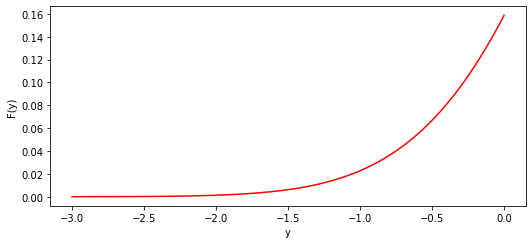
\includegraphics[width=\columnwidth]{figures/F4.png}
    \caption{$F_Y(y)$}
    \label{Fig 3}
    \end{figure}
\end{frame}
\begin{frame}{Probability distribution function}
If $y \ge 0$
    \begin{figure}[h]
    \centering
    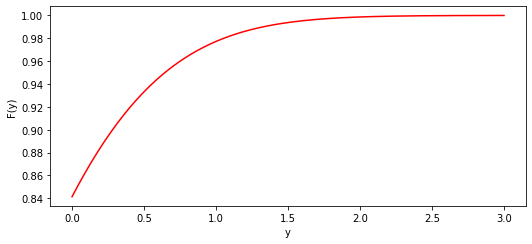
\includegraphics[width=\columnwidth]{figures/F3.png}
    \caption{$F_Y(y)$}
    \label{Fig 4}
    \end{figure}
\end{frame}
\end{document}
